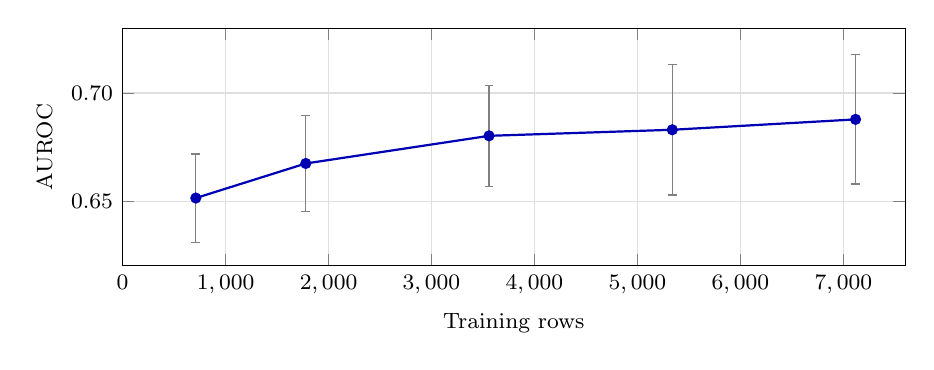
\begin{tikzpicture}
\begin{axis}[width=0.95\columnwidth, height=4.6cm, xlabel={Training rows}, ylabel={AUROC},
  xmin=0, xmax=7600, ymin=0.62, ymax=0.73, label style={font=\footnotesize}, ticklabel style={font=\footnotesize},
  yticklabel style={/pgf/number format/fixed, /pgf/number format/fixed zerofill, /pgf/number format/precision=2},
  scaled x ticks=false, xticklabel style={/pgf/number format/1000 sep={,}}, grid=major, grid style={gray!25}]
\addplot[blue!70!black, thick, mark=*, mark size=1.6pt, error bars/.cd, y dir=both, y explicit, error bar style={gray}] coordinates {(711,0.6514) +- (0,0.0204) (1779,0.6674) +- (0,0.0222) (3559,0.6802) +- (0,0.0233) (5339,0.6830) +- (0,0.0302) (7119,0.6878) +- (0,0.0299)};
\end{axis}
\end{tikzpicture}
